\documentclass[14pt,a4paper]{extarticle}

% ---------- Core Packages ----------
\usepackage[margin=1in]{geometry}
\usepackage{amsmath, amssymb}
\usepackage{enumitem}
\usepackage{titlesec}
\usepackage{float}
\usepackage{booktabs}
\usepackage{hyperref}
\usepackage{xcolor}
\usepackage{tikz}
\usetikzlibrary{arrows.meta, positioning}
\usepackage{tabularx}  % Add this in preamble
% \usepackage{tcolorbox}
\usepackage{longtable}

% ---------- Algorithm ----------
\usepackage{algorithm}
\usepackage{algpseudocode}

% ---------- Listings and Code ----------
\usepackage{listings}
\usepackage{caption}

\usepackage{tikz}
\usepackage{listings}
\usepackage[most]{tcolorbox}

% % ----------------- 
% \bibliography{mcst_references}
% \bibliographystyle{plain}


\definecolor{codegray}{gray}{0.9}
\definecolor{codeblue}{rgb}{0.1,0.1,0.6}
\definecolor{codered}{rgb}{0.6,0.1,0.1}
\definecolor{codegreen}{rgb}{0.1,0.5,0.1}
\definecolor{codeorange}{rgb}{1,0.5,0}

% Code styling
\lstdefinestyle{python}{
  language=Python,
  basicstyle=\ttfamily\small,
  keywordstyle=\color{blue},
  commentstyle=\color{gray},
  stringstyle=\color{orange},
  showstringspaces=false,
  numbers=left,
  numberstyle=\tiny\color{gray},
  breaklines=true,
  frame=single,
  tabsize=4,
  captionpos=b
}

\lstdefinestyle{cpp}{
  language=C++,
  basicstyle=\ttfamily\small,
  keywordstyle=\color{blue},
  commentstyle=\color{gray},
  stringstyle=\color{orange},
  showstringspaces=false,
  numbers=left,
  numberstyle=\tiny\color{gray},
  breaklines=true,
  frame=single,
  tabsize=4,
  captionpos=b
}

% ---------- Hyperref Setup ----------
\hypersetup{
    colorlinks=true,
    linkcolor=black,
    urlcolor=cyan,
    citecolor=blue
}

% ---------- Document Info ----------
\title{Minimum Cost Spanning Trees}
\author{Varun Kumar}
\date{\today}

\begin{document}
\maketitle
\tableofcontents
\lstlistoflistings
% \listofalgorithms
\newpage
\section{Minimum Cost Spanning Tree (MST)}

A \textbf{Spanning Tree} of a connected, undirected graph is a subgraph that includes 
all the vertices with the minimum number of edges (i.e., $V-1$ edges). 
A \textbf{Minimum Cost Spanning Tree} is a spanning tree with the minimum total edge weight.

\subsection*{Applications}
\begin{itemize}
    \item Network design (LAN, telecommunication)
    \item Circuit design
    \item Clustering and approximation algorithms
\end{itemize}

\subsection{Minimum Cost Spanning Tree}

A Minimum Cost Spanning Tree (MCST) connects all vertices of a graph with the smallest possible total edge weight and no cycles.

\subsection{General Approach (Greedy Strategy)}

\begin{algorithm}[H]
\caption{General MCST Algorithm}
\begin{algorithmic}[1]
\State \textbf{Input:} Connected undirected weighted graph \(G = (V, E)\)
\State \textbf{Output:} Set of edges forming the MCST

\Function{MCST}{$G$}
    \State Initialize an empty set \texttt{MST}
    \State Initialize totalCost \( \gets 0 \)
    \While{\texttt{MST} does not have \(V-1\) edges}
        \State Pick the minimum weight edge \( (u, v) \) that doesn't form a cycle in \texttt{MST}
        \State Add \( (u, v) \) to \texttt{MST}
        \State Update totalCost \( \gets \) totalCost $+$ weight of edge
    \EndWhile
    \State \Return \texttt{MST}, totalCost
\EndFunction
\end{algorithmic}
\end{algorithm}

\newpage
\subsection*{Note:}
\begin{itemize}
    \item Step 5 uses cycle detection via DSU (Kruskal) or visited set (Prim).
    \item The greedy approach ensures local optimality leads to global optimality.
\end{itemize}

\subsection*{Explanation of Pseudocode}

The general idea behind the greedy strategy for Minimum Cost Spanning Tree (MCST) is simple and efficient. The algorithm starts with an empty tree and keeps adding the smallest weight edge that does not create a cycle. This process continues until the tree spans all the vertices (i.e., has exactly \(V-1\) edges).

\vspace{1em}
\textbf{Steps Explained in Plain English:}
\begin{itemize}
    \item Start with an empty set to store the MST edges.
    \item Keep track of the total cost (initially zero).
    \item Until we have exactly \(V-1\) edges:
    \begin{itemize}
        \item Look for the smallest edge that connects two different parts of the graph and does not create a cycle.
        \item Add this edge to the MST.
        \item Add its weight to the total cost.
    \end{itemize}
    \item Once the MST has \(V-1\) edges, the algorithm is complete.
    \item Return the final MST and its total cost.
\end{itemize}

\vspace{1em}
This approach is the foundation of well-known algorithms like \textbf{Prim’s} and \textbf{Kruskal’s}, which implement the greedy strategy in different ways.


%%%%%%%%%%%%%%%%%%%%%%%%%% Dynamic Programming Approach %%%%%%%%%%%%%%%%%%%%%%%%%%%%%
\subsection{Dynamic Programming Approach to MCST (Theoretical)}
% \section*{DP-Based Formulation (Bitmask)}

The Minimum Cost Spanning Tree (MCST) problem seeks to connect all vertices of a connected, undirected, 
and weighted graph with the minimum total edge cost, forming a tree (i.e., no cycles). Traditional approaches 
like \textbf{Prim’s} and \textbf{Kruskal’s} algorithms efficiently solve this problem using greedy strategies.

However, from a theoretical perspective, one can formulate MCST as a \textbf{dynamic programming (DP)} 
problem using \textit{bitmasking} to represent subsets of vertices. Although this approach is not practical 
for large graphs due to its exponential time complexity \( O(V^2 \cdot 2^V) \), it provides insight into the 
relationship between combinatorial optimization and DP paradigms.

The DP approach serves as a useful conceptual tool in algorithm theory, NP-completeness discussions, and for 
solving small graph instances in academic contexts.

\begin{algorithm}[H]
\caption{DP approach to MCST (Exponential Time)}
\begin{algorithmic}[1]
\State \textbf{Input:} Graph \( G = (V, E) \)
\State \textbf{Let:} \( dp[S][u] \) = minimum cost to connect subset \( S \subseteq V \) ending at vertex \( u \)
\State Initialize all \( dp[S][u] \gets \infty \)
\For{each vertex \( u \in V \)}
    \State \( dp[2^u][u] \gets 0 \) \Comment{Cost to start at each node}
\EndFor

\For{each subset \( S \subseteq 2^V \)}
    \For{each vertex \( u \in V \) where \( S \) includes \( u \)}
        \For{each neighbor \( v \) of \( u \)}
            \If{\( v \notin S \)}
                \State \( newS \gets S \cup \{v\} \)
                \State \( dp[newS][v] \gets \min(dp[newS][v], dp[S][u] + \text{weight}(u,v)) \)
            \EndIf
        \EndFor
    \EndFor
\EndFor

\State \Return \( \min_{u} dp[2^V - 1][u] \)
\end{algorithmic}
\end{algorithm}

\subsection*{Note}
This algorithm is exponential and mainly of theoretical interest.
For practical purposes, Prim’s or Kruskal’s algorithm is always preferred.

\newpage
\subsection*{DP Approach to MCST (Exponential Time)}

This algorithm uses a Dynamic Programming (DP) approach to find the Minimum Cost Spanning Tree (MCST). It is based on the idea of exploring all subsets of vertices and building the solution incrementally. Although not efficient for large graphs (exponential time), it is conceptually useful and similar in spirit to the Held-Karp algorithm for TSP.

\vspace{1em}
\textbf{Plain English Explanation of the Algorithm:}
\begin{itemize}
    \item The graph is represented as \(G = (V, E)\), where \(V\) is the set of vertices and \(E\) is the set of edges.
    \item Define a DP table: \texttt{dp[S][u]} represents the minimum cost to connect all vertices in subset \(S \subseteq V\), ending at vertex \(u\).
    \item Initially, set all \texttt{dp[S][u]} to \(\infty\) (unknown or unreachable).
    \item For each vertex \(u\), set \texttt{dp[\{u\}][u] = 0}, meaning starting at node \(u\) with only that node in the subset has zero cost.
    \item For all subsets \(S\) of vertices:
    \begin{itemize}
        \item For each vertex \(u\) in subset \(S\):
        \begin{itemize}
            \item For each neighbor \(v\) of \(u\) that is not already in \(S\):
            \begin{itemize}
                \item Let \texttt{newS = S \textbackslash{}cup \{\{v\}\}}, which means \(S \cup \{v\}\).
                \item Update the DP value for \texttt{dp[newS][v]} as the minimum of its current value or the cost of extending \texttt{dp[S][u]} by the edge \((u,v)\).
            \end{itemize}
        \end{itemize}
    \end{itemize}
    \item After all subsets have been processed, the final answer is the minimum of \texttt{dp[2\^{}V - 1][u]} over all \(u\), which represents the cost to connect all nodes, ending at any node \(u\).
\end{itemize}


\vspace{1em}
\textbf{Note:} This algorithm runs in exponential time, \(O(V \cdot 2^V)\), and is used mainly for theoretical or very small graphs.

\newpage
\subsection{When to Use Dynamic Programming for Minimum Cost Spanning Tree (MCST)}

Dynamic Programming (DP) is generally not the most efficient method for solving MCST problems in practice. However, it becomes relevant in:

\begin{itemize}
    \item \textbf{Theoretical analysis:} DP helps in understanding the structure and properties of spanning trees and optimal substructure.
    \item \textbf{Special versions:} Problems like the \textit{Travelling Salesman Problem (TSP)} or \textit{Steiner Tree}, which are extensions or variants of MCST, often require DP.
    \item \textbf{Exhaustive optimization:} When all possible spanning trees need to be analyzed (e.g., for robustness or reliability), DP can be used to cache results and reduce recomputation.
    \item \textbf{Dynamic Graphs:} If the graph changes (edge insertions/deletions), certain DP-based or memoization strategies can help update the MCST incrementally.
\end{itemize}

\noindent
In general, greedy algorithms like \textbf{Prim’s} and \textbf{Kruskal’s} are preferred due to their simplicity and efficiency, but DP is valuable when the problem cannot be solved optimally using greedy methods alone.


%%%%%%%%%%%%%%%%%%%%%%%%%%%%%%%%%%%%%%%%%%%% Prim's Algorithm %%%%%%%%%%%%%%%%%%%%%%%%%%%%%%%%%%%%
\newpage
\section{Prim's Algorithm}

Prim's\cite{prim1957} algorithm grows the MST one edge at a time, starting from an arbitrary node. 
It always adds the minimum weight edge that connects a visited node to an unvisited node.



\subsection{Algorithm Steps}
\begin{itemize}
    \item Initialize a priority queue (min-heap) with the starting vertex.
    \item Repeat until all vertices are included:
    \begin{itemize}
        \item Extract the edge with minimum weight.
        \item If the adjacent node is unvisited, add it to the MST.
    \end{itemize}
\end{itemize}

%%%%%%%%%%%%%%%%%%%%%%%%%%%%%%%%%%%%%%%%%%%%%%%%%%%%%%%%%%%%%%%%%%%%%%%%%%%%%%%%%%%%%%%
\subsection{Core Idea}
Prim's Algorithm constructs a Minimum Spanning Tree (MST) by:
\begin{itemize}
    \item Starting from an arbitrary node.
    \item Maintaining a priority queue to track minimum weight edges.
    \item At each step, selecting the smallest edge that connects the MST to a new vertex.
    \item Repeating until all vertices are included.
\end{itemize}

\section*{Pseudocode}

\begin{algorithm}[H]
\caption{Prim's Algorithm}
\begin{algorithmic}[1]
\State \textbf{Input:} Weighted undirected graph $G = (V, E)$
\State \textbf{Output:} Minimum Cost of Spanning Tree

\Function{Prim}{Graph $G$, Start Vertex $s$}
    \State Initialize a min-heap $Q$
    \State $visited \gets$ empty set
    \State $cost \gets 0$
    \State Insert $(0, s)$ into $Q$ \Comment{Start with source node}

    \While{$Q$ is not empty}
        \State $(w, u) \gets$ Extract-Min from $Q$
        \If{$u \notin visited$}
            \State Add $u$ to $visited$
            \State $cost \gets cost + w$
            \For{each neighbor $(v, weight)$ of $u$}
                \If{$v \notin visited$}
                    \State Insert $(weight, v)$ into $Q$
                \EndIf
            \EndFor
        \EndIf
    \EndWhile

    \State \Return $cost$
\EndFunction
\end{algorithmic}
\end{algorithm}
%%%%%%%%%%%%%%%%%%%%%%%%%%%%%%%%%%%%%%%%%%%%%%%%%%%%%%%%%%%%%%%%%%%%%%%%%%%%%%%%%%%%%%%

\subsection*{Time and Space Complexity}
\begin{itemize}
    \item Time: $O(E \log V)$ with min-heap and adjacency list
    \item Space: $O(V)$
\end{itemize}

%%%%%%%%%%%%%%%%%%%%%%%%%% Dry Run Example %%%%%%%%%%%%%%%%%%%%%%%%%%%%%
\newpage
\subsection{Prim's Algorithm: Step-by-Step Dry Run Example}

\textbf{Graph:}

\tcbset{colback=white, colframe=black, boxrule=0.5pt, arc=4pt}

\begin{tcolorbox}[title=Directed Weighted Graph]

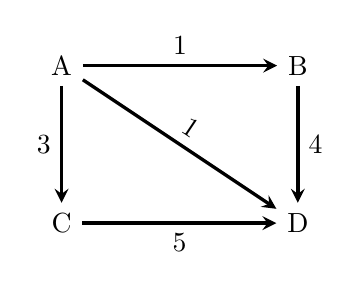
\begin{tikzpicture}[
    ->, >=stealth, auto, node distance=2cm,
    vertex/.style={circle, draw, minimum size=7mm, font=\small},
    edge label/.style={font=\footnotesize, inner sep=1pt},
    line width=1.2pt, draw=black
]


\node (A) at (0,0) {A};
\node (B) at (3,0) {B};
\node (C) at (0,-2) {C};
\node (D) at (3,-2) {D};

\draw (A) -- (B) node[midway, above] {1};
\draw (A) -- (C) node[midway, left] {3};
\draw (A) -- (D) node[midway, sloped, above] {1};
\draw (B) -- (D) node[midway, right] {4};
\draw (C) -- (D) node[midway, below] {5};


\end{tikzpicture}
\end{tcolorbox}


\subsection*{Step-by-Step Execution (Start from A)}

\begin{longtable}{|c|p{8cm}|}
\hline
\textbf{Step} & \textbf{Action and Explanation} \\
\hline
1 & Start at vertex A. Add A to visited set. Insert its neighbors (B, 1), (C, 3), (D, 1) into priority queue. \\
\hline
2 & Extract min edge (A–B, 1). B is unvisited. Add B to MST and visited set. Push B’s neighbor (D, 4). Queue now: (D, 1), (C, 3), (D, 4) \\
\hline
3 & Extract min edge (A–D, 1). D is unvisited. Add D to MST. Push its neighbor (C, 5). Queue now: (C, 3), (D, 4), (C, 5) \\
\hline
4 & Extract min edge (A–C, 3). C is unvisited. Add C to MST. All vertices visited. \\
\hline
\end{longtable}

\subsection*{Final MST Edges and Cost}

\begin{itemize}
    \item Edges in MST: (A–B, 1), (A–D, 1), (A–C, 3)
    \item Total Cost = $1 + 1 + 3 = 5$
\end{itemize}

%%%%%%%%%%%%%%%%%%%%%%%%%%%% Python and C++ Code %%%%%%%%%%%%%%%%%%%%%%%%%%%%%
\newpage
\subsection{Python Code}
\begin{lstlisting}[style=python, caption={Prim's Algorithm in Python}]
import heapq

def prim(graph, start):
    visited = set()
    min_heap = [(0, start)]
    mst_cost = 0

    while min_heap:
        weight, u = heapq.heappop(min_heap)
        if u not in visited:
            visited.add(u)
            mst_cost += weight
            for v, w in graph[u]:
                if v not in visited:
                    heapq.heappush(min_heap, (w, v))

    return mst_cost
\end{lstlisting}

\subsection{C++ Code}
\begin{lstlisting}[style=cpp, caption={Prim's Algorithm in C++}]
#include <bits/stdc++.h>
using namespace std;

int prim(vector<vector<pair<int,int>>> &graph, int V) {
    vector<bool> visited(V, false);
    priority_queue<pair<int,int>, vector<pair<int,int>>, greater<>> pq;
    pq.push({0, 0});
    int cost = 0;

    while (!pq.empty()) {
        auto [w, u] = pq.top(); pq.pop();
        if (!visited[u]) {
            visited[u] = true;
            cost += w;
            for (auto [v, wt] : graph[u])
                if (!visited[v])
                    pq.push({wt, v});
        }
    }
    return cost;
}
\end{lstlisting}

\newpage
%%%%%%%%%%%%%%%%%%%%%%%%%%%%%%%%%%%%%%%%%%%%%%%%%%%%%%%%%%%%%%%%%%%%%%%%%%%%%%%%%%%%%%%%%%%%%%
%%%%%%%%%%%%%%%%%%%%%%%%%%%%%%%%%%%%% Kruskal's Algorithm %%%%%%%%%%%%%%%%%%%%%%%%%%%%%%%%%%%%
%%%%%%%%%%%%%%%%%%%%%%%%%%%%%%%%%%%%%%%%%%%%%%%%%%%%%%%%%%%%%%%%%%%%%%%%%%%%%%%%%%%%%%%%%%%%%%
\section{Kruskal's Algorithm} 

Kruskal's\cite{kruskal1956} algorithm sorts all edges in increasing order and adds them one by one to the MST if 
they do not form a cycle. It uses the Disjoint Set Union (DSU) data structure.

\subsection{Algorithm Steps}
\begin{itemize}
    \item Sort all edges in ascending order.
    \item Initialize each node as its own set.
    \item Iterate through the edges and add them to the MST if they connect different sets.
\end{itemize}

\subsection{Core Idea}
\begin{itemize}
    \item Sort all edges in increasing order of weight.
    \item Use the \textbf{Disjoint Set Union (DSU)} data structure to detect cycles.
    \item Keep adding the next lightest edge that doesn't cause a cycle.
    \item Stop when \(V-1\) edges have been added (where \(V\) is the number of vertices).
\end{itemize}

\subsection*{Time and Space Complexity}
\begin{itemize}
    \item \textbf{Time Complexity:} \(O(E \log E)\), dominated by sorting and union-find operations.
    \item \textbf{Space Complexity:} \(O(V)\) for DSU.
\end{itemize}

\subsection{Pseudocode}

\begin{algorithm}[H]
\caption{Kruskal's Algorithm}
\begin{algorithmic}[1]
\State \textbf{Input:} Graph \(G = (V, E)\)
\State \textbf{Output:} MST set of edges

\Function{Kruskal}{V, E}
    \State Sort edges \(E\) in ascending order by weight
    \State Initialize DSU with each vertex in its own set
    \State MSTEdges \(\gets\) empty set

    \For{each edge \((u, v)\) in sorted \(E\)}
        \If{\Call{Find}{u} \(\ne\) \Call{Find}{v}}
            \State Add \((u, v)\) to MSTEdges
            \State \Call{Union}{u, v}
        \EndIf
    \EndFor

    \State \Return MSTEdges
\EndFunction

\Function{Find}{x}
    \If{parent[x] \(\ne\) x}
        \State parent[x] \(\gets\) \Call{Find}{parent[x]} \Comment{Path compression}
    \EndIf
    \State \Return parent[x]
\EndFunction

\Function{Union}{x, y}
    \State xRoot \(\gets\) \Call{Find}{x}
    \State yRoot \(\gets\) \Call{Find}{y}
    \If{rank[xRoot] < rank[yRoot]}
        \State parent[xRoot] \(\gets\) yRoot
    \ElsIf{rank[yRoot] < rank[xRoot]}
        \State parent[yRoot] \(\gets\) xRoot
    \Else
        \State parent[yRoot] \(\gets\) xRoot
        \State rank[xRoot] \(\gets\) rank[xRoot] + 1
    \EndIf
\EndFunction
\end{algorithmic}
\end{algorithm}


%%%%%%%%%%%%%%%%%%%%%%%%%%%%%%%%%%%%%%%%%%%%%%%%%%%%%%%%%%%%%%%%%%%%%%%%%%%%
%%%%%%%%%%%%%%%%%%%%%%%% Working Example %%%%%%%%%%%%%%%%%%%%%%%%%%%%%%%%%%%
%%%%%%%%%%%%%%%%%%%%%%%%%%%%%%%%%%%%%%%%%%%%%%%%%%%%%%%%%%%%%%%%%%%%%%%%%%%%
\newpage
\subsection{Dry Run Example: Kruskal’s Algorithm}

\textbf{Graph:}

\tcbset{colback=white, colframe=black, boxrule=0.5pt, arc=4pt}

\begin{tcolorbox}[title=Directed Weighted Graph]

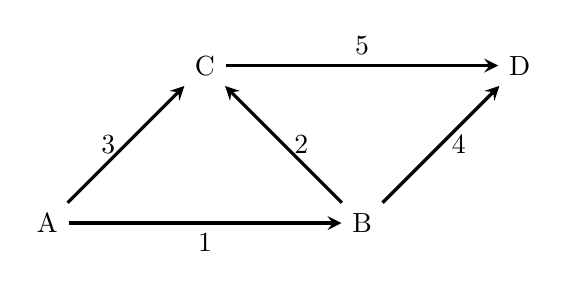
\begin{tikzpicture}[
    ->, >=stealth, auto, node distance=2cm,
    vertex/.style={circle, draw, minimum size=7mm, font=\small},
    edge label/.style={font=\footnotesize, inner sep=1pt},
    line width=1.2pt, draw=black
]


\node (A) at (0,0) {A};
\node (B) at (4,0) {B};
\node (C) at (2,2) {C};
\node (D) at (6,2) {D};

\draw (A) -- (B) node[midway,below] {1};
\draw (A) -- (C) node[midway,left] {3};
\draw (B) -- (C) node[midway,right] {2};
\draw (B) -- (D) node[midway,right] {4};
\draw (C) -- (D) node[midway,above] {5};


\end{tikzpicture}
\end{tcolorbox}

\textbf{Vertices:} A, B, C, D \hfill \textbf{Edges:} 5

\vspace{1em}
\textbf{Step 1: Sort edges by weight}

\begin{itemize}
  \item (A--B, 1)
  \item (B--C, 2)
  \item (A--C, 3)
  \item (B--D, 4)
  \item (C--D, 5)
\end{itemize}

\vspace{1em}
\textbf{Step 2: Initialize DSU}

\begin{center}
\begin{tabular}{|c|c|}
\hline
Vertex & Parent \\
\hline
A & A \\
B & B \\
C & C \\
D & D \\
\hline
\end{tabular}
\end{center}

\vspace{1em}
\textbf{Step 3: Process edges one by one}

\begin{itemize}
  \item \textbf{(A--B, 1)}: Find(A) = A, Find(B) = B $\Rightarrow$ Different sets $\Rightarrow$ Add edge to MST  
  \quad $\Rightarrow$ Union(A, B) $\Rightarrow$ Parent[B] = A

  \item \textbf{(B--C, 2)}: Find(B) = A, Find(C) = C $\Rightarrow$ Different $\Rightarrow$ Add to MST  
  \quad $\Rightarrow$ Union(B, C) $\Rightarrow$ Parent[C] = A

  \item \textbf{(A--C, 3)}: Find(A) = A, Find(C) = A $\Rightarrow$ Same set $\Rightarrow$ Ignore (would form cycle)

  \item \textbf{(B--D, 4)}: Find(B) = A, Find(D) = D $\Rightarrow$ Different $\Rightarrow$ Add to MST  
  \quad $\Rightarrow$ Union(B, D) $\Rightarrow$ Parent[D] = A

  \item \textbf{(C--D, 5)}: Find(C) = A, Find(D) = A $\Rightarrow$ Same set $\Rightarrow$ Ignore
\end{itemize}


\vspace{1em}
\textbf{Final MST:}
\begin{itemize}
  \item (A--B, 1)
  \item (B--C, 2)
  \item (B--D, 4)
\end{itemize}

\textbf{Total Cost:} \(1 + 2 + 4 = 7\)

\vspace{1em}
\textbf{Final DSU Table:}

\begin{center}
\begin{tabular}{|c|c|}
\hline
Vertex & Parent \\
\hline
A & A \\
B & A \\
C & A \\
D & A \\
\hline
\end{tabular}
\end{center}

%%%%%%%%%%%%%%%%%%%%%%%%%%%%%%%%%%%%%%%%%%%%%%%%%%%%%%%%%%%%%%%%%%%%%%%%%%%%%%%%%%%%%%
% def find(parent, x):
%     if parent[x] != x:
%         parent[x] = find(parent, parent[x])
%     return parent[x]

% def union(parent, rank, x, y):
%     xroot = find(parent, x)
%     yroot = find(parent, y)
%     if xroot != yroot:
%         if rank[xroot] < rank[yroot]:
%             parent[xroot] = yroot
%         else:
%             parent[yroot] = xroot
%             if rank[xroot] == rank[yroot]:
%                 rank[xroot] += 1

% def kruskal(V, edges):
%     edges.sort(key=lambda x: x[2])
%     parent = list(range(V))
%     rank = [0]*V
%     cost = 0

%     for u, v, w in edges:
%         if find(parent, u) != find(parent, v):
%             union(parent, rank, u, v)
%             cost += w

%     return cost
%%%%%%%%%%%%%%%%%%%%%%%%%%%%%%%%%%%%%%%%%%%%%%%%%%%%%%%%%%%%%%%%%%%%%%%%%%%%%%%%%%%%%%

\newpage
\subsection{Python Code}
\begin{lstlisting}[style=python, caption={Kruskal's Algorithm in Python}]
def find(parent, x):
    if parent[x] != x:
        parent[x] = find(parent, parent[x])  # Path compression
    return parent[x]

def union(parent, rank, x, y):
    xroot = find(parent, x)
    yroot = find(parent, y)
    if xroot != yroot:
        if rank[xroot] < rank[yroot]:
            parent[xroot] = yroot
        else:
            parent[yroot] = xroot
            if rank[xroot] == rank[yroot]:
                rank[xroot] += 1

def kruskal(V, edges):
    edges.sort(key=lambda x: x[2])  # Sort by weight
    parent = list(range(V))
    rank = [0] * V
    cost = 0

    for u, v, w in edges:
        if find(parent, u) != find(parent, v):
            union(parent, rank, u, v)
            cost += w

    return cost

# ===========================
# User Input Section
# ===========================

V, E = map(int, input("Enter number of vertices and edges: ").split())
edges = []

print("Enter edges in format: u v w (0-indexed)")
for _ in range(E):
    u, v, w = map(int, input().split())
    edges.append((u, v, w))

# Run Kruskal's Algorithm
mst_cost = kruskal(V, edges)
print("Minimum Cost of Spanning Tree:", mst_cost)
\end{lstlisting}

\begin{verbatim}
# Number of vertices
V = 4
# List of edges (u, v, weight)
edges = [
    (0, 1, 10),
    (0, 2, 6),
    (0, 3, 5),
    (1, 3, 15),
    (2, 3, 4)
]
# Run Kruskal's algorithm and print MST cost
print("Minimum Cost of Spanning Tree:", kruskal(V, edges))

\end{verbatim}

%%%%%%%%%%%%%%%%%%%%%% End Python Code %%%%%%%%%%%%%%%%%%%%%%%%%%%%%%

\subsection{Working of Kruskal's Algorithm (Python)}

\subsection*{Dry Run Example}

\begin{tcolorbox}[title=Graph Details]
Vertices: 4 (0, 1, 2, 3)\\
Edges:\\
(0, 1, 10), (0, 2, 6), (0, 3, 5), (1, 3, 15), (2, 3, 4)
\end{tcolorbox}
4 Vertices with lebels 0, 1, 2, 3 and edges with weights as follows:
between 0 and 1 = 10, between 0 and 2 = 6, between 0 and 3 = 5, between 1 and 3 = 15, between 2 and 3 = 4.
\subsubsection*{Step 1: Sort Edges by Weight}
\begin{itemize}
    \item (2, 3, 4)
    \item (0, 3, 5)
    \item (0, 2, 6)
    \item (0, 1, 10)
    \item (1, 3, 15)
\end{itemize}

\subsubsection*{Step 2: Initialize}
\begin{itemize}
    \item parent = [0, 1, 2, 3]
    \item rank = [0, 0, 0, 0]
    \item cost = 0
\end{itemize}

\subsubsection*{Step 3: Process Each Edge}
\begin{itemize}
    \item \textbf{(2, 3, 4)}: Find(2)=2, Find(3)=3 → Different sets → Add to MST\\
    \quad Union(2, 3) → parent[3] = 2 → cost = 4

    \item \textbf{(0, 3, 5)}: Find(0)=0, Find(3)=Find(2)=2 → Different sets → Add to MST\\
    \quad Union(0, 2) → parent[2] = 0 → cost = 9

    \item \textbf{(0, 2, 6)}: Find(0)=0, Find(2)=Find(0)=0 → Same set → Ignore

    \item \textbf{(0, 1, 10)}: Find(0)=0, Find(1)=1 → Different sets → Add to MST\\
    \quad Union(0, 1) → parent[1] = 0 → cost = 19

    \item \textbf{(1, 3, 15)}: Find(1)=Find(0)=0, Find(3)=Find(2)=Find(0)=0 → Same set → Ignore
\end{itemize}

\subsubsection*{Final MST}
Edges included in MST:
\begin{itemize}
    \item (2, 3, 4)
    \item (0, 3, 5)
    \item (0, 1, 10)
\end{itemize}
Total cost of MST = \textbf{19}

\subsection*{Edge Inclusion Summary}
\begin{center}
\begin{tabular}{|c|c|c|}
\hline
\textbf{Edge} & \textbf{Included in MST?} & \textbf{Reason} \\
\hline
(2, 3, 4) & Yes & Different sets \\
(0, 3, 5) & Yes & Different sets \\
(0, 2, 6) & No & Same set (would form cycle) \\
(0, 1, 10) & Yes & Different sets \\
(1, 3, 15) & No & Same set (would form cycle) \\
\hline
\end{tabular}
\end{center}

%%%%%%%%%%%%%%%%%%%%%%%%%%%%%%% C++ Code %%%%%%%%%%%%%%%%%%%%%%%%%%%%%%
\newpage
\subsection{C++ Code}
\begin{lstlisting}[style=cpp, caption={Kruskal's Algorithm in C++}]
struct Edge {
    int u, v, w;
    bool operator<(const Edge& e) const { return w < e.w; }
};

int find(int parent[], int x) {
    if (parent[x] != x)
        parent[x] = find(parent, parent[x]);
    return parent[x];
}

void unite(int parent[], int rank[], int x, int y) {
    int xroot = find(parent, x);
    int yroot = find(parent, y);
    if (rank[xroot] < rank[yroot])
        parent[xroot] = yroot;
    else {
        parent[yroot] = xroot;
        if (rank[xroot] == rank[yroot]) rank[xroot]++;
    }
}

int kruskal(int V, vector<Edge>& edges) {
    sort(edges.begin(), edges.end());
    int parent[V], rank[V] = {};
    iota(parent, parent + V, 0);
    int cost = 0;

    for (auto& e : edges) {
        if (find(parent, e.u) != find(parent, e.v)) {
            unite(parent, rank, e.u, e.v);
            cost += e.w;
        }
    }
    return cost;
}
\end{lstlisting}

\newpage
%%%%%%%%%%%%%%%%%%%%%%%%%%%%%%%%%%%%%%%%%%%%%%%%%%%%%%%%%%%%%%%%%%%%%%%%%%%%%%%%%%%%%%%%%%%%%%
%%%%%%%%%%%%%%%%%%%%%%%%%%%%%%%%%%%% Dijkstra's Algorithm %%%%%%%%%%%%%%%%%%%%%%%%%%%%%%%%%%%%
%%%%%%%%%%%%%%%%%%%%%%%%%%%%%%%%%%%%%%%%%%%%%%%%%%%%%%%%%%%%%%%%%%%%%%%%%%%%%%%%%%%%%%%%%%%%%%
\section{Dijkstra's Algorithm (Shortest Path, Not MST)}

\textbf{Note:} Dijkstra's Algorithm is not used to compute MST. It is used for finding the shortest path from a source node to all other nodes in a graph with non-negative weights.

\subsection*{Steps}
\begin{itemize}
    \item Use a priority queue to pick the node with the least distance.
    \item Update distances of adjacent vertices if a shorter path is found.
\end{itemize}

\subsection*{Time and Space Complexity}
\begin{itemize}
    \item Time: $O(E \log V)$
    \item Space: $O(V)$
\end{itemize}

\subsection{Dijkstra's Algorithm: Logic}
\subsection*{Purpose}
Dijkstra’s algorithm is used to \textbf{find the shortest path} from a \textbf{source node} to all other nodes in a \textbf{weighted graph} with \textbf{non-negative edge weights}.

\subsection*{Core Idea (Greedy Approach)}
\begin{itemize}
    \item Start from the source vertex.
    \item At each step, \textbf{select the node with the smallest known distance} from the source (greedy choice).
    \item \textbf{Update distances} of its neighbors if shorter paths are found.
    \item Repeat until all vertices are processed.
\end{itemize}

\subsection*{Working Steps}
\begin{enumerate}
    \item Initialize all distances to $\infty$ except the source (set to 0).
    \item Use a min-priority queue (or min-heap) to pick the vertex with the \textbf{minimum distance}.
    \item For each neighbor $v$ of current node $u$, if 
    \[
    \text{dist}[u] + \text{weight}(u, v) < \text{dist}[v]
    \]
    then update $\text{dist}[v]$.
    \item Continue until all vertices are visited.
\end{enumerate}

\subsection{Dijkstra’s Algorithm Pseudocode}
\begin{algorithm}[H]
\caption{Dijkstra’s Algorithm}
\begin{algorithmic}[1]
\Procedure{Dijkstra}{$G, source$}
    \State Initialize distance array $dist[v] \gets \infty$ for all $v$ in $G$
    \State $dist[source] \gets 0$
    \State Create a min-priority queue $Q$
    \State $Q.\text{insert}(source, 0)$

    \While{$Q$ is not empty}
        \State $u \gets Q.\text{extract\_min}()$
        \ForAll{neighbors $v$ of $u$}
            \If{$dist[u] + weight(u, v) < dist[v]$}
                \State $dist[v] \gets dist[u] + weight(u, v)$
                \State $Q.\text{insert\_or\_update}(v, dist[v])$
            \EndIf
        \EndFor
    \EndWhile

    \State \Return $dist$
\EndProcedure
\end{algorithmic}
\end{algorithm}

%%%%%%%%%%%%%%%%5 Working Example %%%%%%%%%%%%%%%%%%%%
\newpage
\subsection{Dijkstra’s Algorithm: Worked Example}

\subsection*{Sample Graph}
Consider the following weighted, undirected graph with 5 nodes:

\tcbset{colback=white, colframe=black, boxrule=0.5pt, arc=4pt}

\begin{tcolorbox}[title=Directed Weighted Graph]

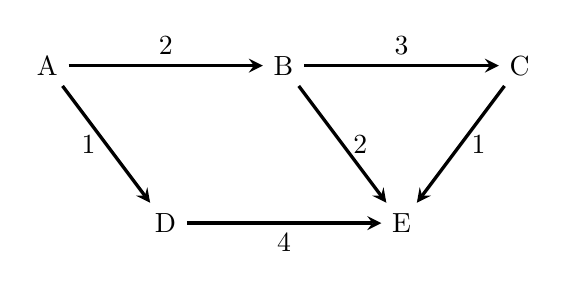
\begin{tikzpicture}[
    ->, >=stealth, auto, node distance=2cm,
    vertex/.style={circle, draw, minimum size=7mm, font=\small},
    edge label/.style={font=\footnotesize, inner sep=1pt},
    line width=1.2pt, draw=black
]


\node (A) at (0,0) {A};
\node (B) at (3,0) {B};
\node (C) at (6,0) {C};
\node (D) at (1.5,-2) {D};
\node (E) at (4.5,-2) {E};

\draw (A) -- (B) node[midway, above] {2};
\draw (B) -- (C) node[midway, above] {3};
\draw (A) -- (D) node[midway, left] {1};
\draw (D) -- (E) node[midway, below] {4};
\draw (B) -- (E) node[midway, right] {2};
\draw (C) -- (E) node[midway, right] {1};
\end{tikzpicture}

\end{tcolorbox}

\textbf{Goal:} Find the shortest distances from source node A to all other nodes.

\subsection*{Initialization}
\begin{itemize}
    \item Set distance of A = 0, all others = $\infty$
    \item Distance array: \texttt{dist = \{A:0, B:$\infty$, C:$\infty$, D:$\infty$, E:$\infty$\}}
    \item Min-heap queue: \texttt{Q = [(0, A)]}
\end{itemize}

\subsection*{Step-by-Step Execution}

\begin{enumerate}
    \item \textbf{Extract A (0):}
    \begin{itemize}
        \item Neighbors: B (2), D (1)
        \item Update dist[B] = 2, dist[D] = 1
        \item Q = [(1, D), (2, B)]
    \end{itemize}

    \item \textbf{Extract D (1):}
    \begin{itemize}
        \item Neighbors: A (already visited), E (1+4=5)
        \item Update dist[E] = 5
        \item Q = [(2, B), (5, E)]
    \end{itemize}

    \item \textbf{Extract B (2):}
    \begin{itemize}
        \item Neighbors: A, C (2+3=5), E (2+2=4)
        \item Update dist[C] = 5, dist[E] = \textbf{min(5,4)=4}
        \item Q = [(4, E), (5, C)]
    \end{itemize}

    \item \textbf{Extract E (4):}
    \begin{itemize}
        \item Neighbors: D, B, C (4+1=5) → No change
        \item Q = [(5, C)]
    \end{itemize}

    \item \textbf{Extract C (5):} All neighbors visited. Done.
\end{enumerate}

\subsection*{Final Shortest Distances from A}
\begin{center}
\begin{tabular}{|c|c|}
\hline
\textbf{Node} & \textbf{Distance from A} \\
\hline
A & 0 \\
B & 2 \\
C & 5 \\
D & 1 \\
E & 4 \\
\hline
\end{tabular}
\end{center}

\subsection*{Path Summary}
\begin{itemize}
    \item A $\rightarrow$ D = 1
    \item A $\rightarrow$ B = 2
    \item A $\rightarrow$ B $\rightarrow$ E = 4
    \item A $\rightarrow$ B $\rightarrow$ C = 5
\end{itemize}

\textbf{Note:} The greedy nature of Dijkstra ensures the shortest path is computed correctly as long as edge weights are non-negative.

%%%%%%%%%%%%%%%%% Ends Here %%%%%%%%%%%%%%%%%%%%


\newpage
\subsection*{Python Code}
\begin{lstlisting}[style=python, caption={Dijkstra’s Algorithm in Python}]
import heapq

def dijkstra(graph, start):
    dist = {node: float('inf') for node in graph}
    dist[start] = 0
    pq = [(0, start)]

    while pq:
        d, u = heapq.heappop(pq)
        if d > dist[u]: continue
        for v, w in graph[u]:
            if dist[u] + w < dist[v]:
                dist[v] = dist[u] + w
                heapq.heappush(pq, (dist[v], v))
    return dist
\end{lstlisting}

\subsection*{C++ Code}
\begin{lstlisting}[style=cpp, caption={Dijkstra’s Algorithm in C++}]
#include <bits/stdc++.h>
using namespace std;

vector<int> dijkstra(int V, vector<pair<int,int>> adj[]) {
    vector<int> dist(V, INT_MAX);
    dist[0] = 0;
    priority_queue<pair<int,int>, vector<pair<int,int>>, greater<>> pq;
    pq.push({0, 0});

    while (!pq.empty()) {
        auto [d, u] = pq.top(); pq.pop();
        for (auto [v, w] : adj[u]) {
            if (dist[u] + w < dist[v]) {
                dist[v] = dist[u] + w;
                pq.push({dist[v], v});
            }
        }
    }
    return dist;
}
\end{lstlisting}
%%%%%%%%%%%%%%%%%%%%%%%%%%%%% Code Ends Here %%%%%%%%%%%%%%%%%%%%%%%%%%%%%%%

%%%%%%%%%%%%%%%%%% GATE CSE Question %%%%%%%%%%%%%%%%%%%%%%

%%%%%%%%%%%%%%%%%%%% 2004 Question %%%%%%%%%%%%%%%%%%%%%%
% Direct application of Dijkstra's algorithm (shortest path calculation).
\newpage
\subsection{GATE CSE 2004}
Suppose we run Dijkstra’s single source shortest path algorithm on the 
following edge-weighted directed graph with vertex $P$ as the source.

\tcbset{colback=white, colframe=black, boxrule=0.5pt, arc=4pt}

\begin{tcolorbox}[title=Directed Weighted Graph]

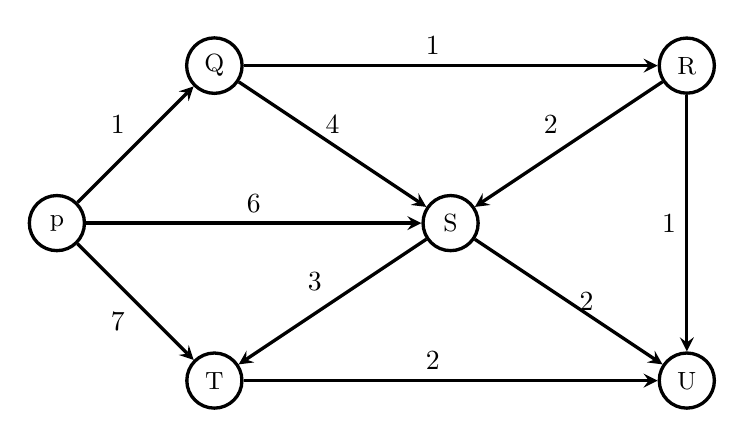
\begin{tikzpicture}[
    ->, >=stealth, auto, node distance=2cm,
    vertex/.style={circle, draw, minimum size=7mm, font=\small},
    edge label/.style={font=\footnotesize, inner sep=1pt},
    line width=1.2pt, draw=black
]
% Nodes
\node[vertex] (P) at (0,0) {p};
\node[vertex] (Q) at (2,2) {Q};
\node[vertex] (T) at (2, -2) {T};
\node[vertex] (S) at (5, 0) {S};
\node[vertex] (R) at (8, 2) {R};
\node[vertex] (U) at (8,-2) {U};

\draw (P) -- (Q) node[midway, above left] {1};
\draw (P) -- (T) node[midway, below left] {7};
\draw (P) -- (S) node[midway, above] {6};

\draw (Q) -- (R) node[midway, above left] {1};
\draw (Q) -- (S) node[midway, above] {4};

\draw (R) -- (S) node[midway, above left] {2};
\draw (R) -- (U) node[midway, left] {1};

\draw (S) -- (T) node[midway, above left] {3};
\draw (S) -- (U) node[midway, right] {2};

\draw (T) -- (U) node[midway, above left] {2};

\end{tikzpicture}

\end{tcolorbox}

\begin{tabular}{ll}
(a) P, Q, R, S, T, U \hspace{4cm} & (b) P, Q, R, U, S, T \\
(c) P, Q, R, U, T, S \hspace{4cm} & (d) P, Q, T, R, U, S \\
\end{tabular}
\vspace{0.5cm}

\url{https://gateoverflow.in/1041/gate-cse-2004-question-44}

%%%%%%%%%%%%%%%%%%% 2005 Question %%%%%%%%%%%%%%%%%%%%%%
% Time complexity of Dijkstra's Algorithm
\subsection{GATE CSE 2005}
Let $G(V, e)$ an undirected graph with positive edge weights. Dijkstra's Single Source
Shortest Path algorithm can be implemented using the binary heap data structure with 
time complexity of?
\subsubsection*{}
\begin{tabular}{ll}
(a) $O\left(|V|^2\right)$ \hspace{4cm} & (b) $O\left(|E|+|V|\log |V|\right)$ \\
(c) $O\left(|V|\log|V|\right)$ \hspace{4cm} & (d) $O\left(\left(|E|+|V|\right)\log|V|\right)$ \\
\end{tabular}
\vspace{0.5cm}

\url{https://gateoverflow.in/1374/gate-cse-2005-question-38}


%%%%%%%%%%%%%%%%%%%% 2012 Question %%%%%%%%%%%%%%%%%%%%%%
\newpage
\subsection{GATE CSE 2012}
Consider the directed graph shown in the figure below. There are 
multiple shortest path between vertices S and T. Which one 
will be reported by Dijkstra's Shortest Path algorithm?
Assume that, in any iteration, the shortest path to a vertex v is 
updated only when a strictly shorter path to v is 
discovered.

\tcbset{colback=white, colframe=black, boxrule=0.5pt, arc=4pt}

\begin{tcolorbox}[title=Directed Weighted Graph]

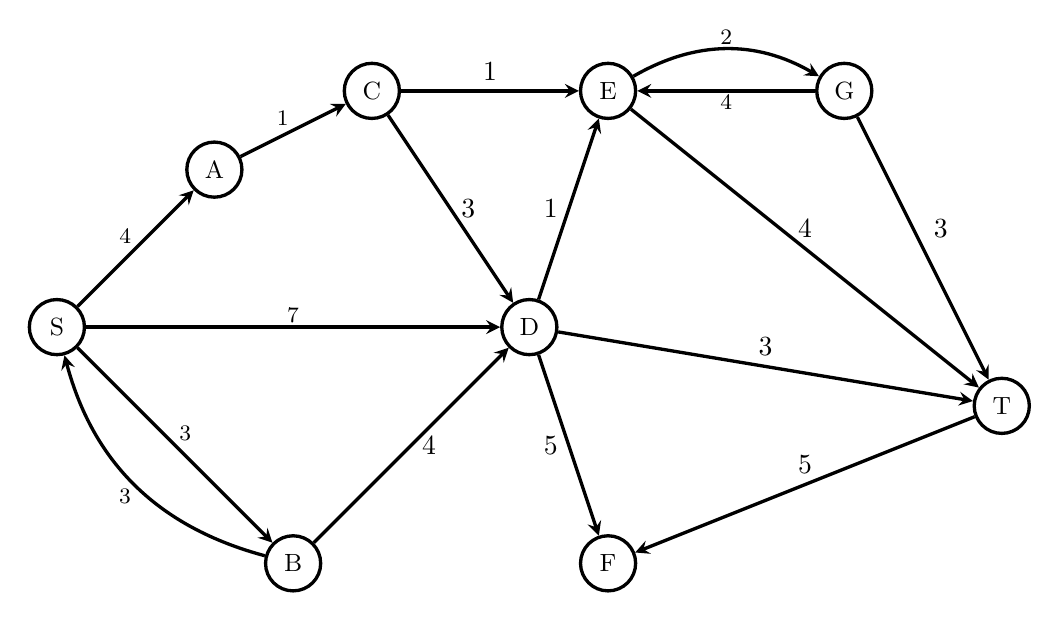
\begin{tikzpicture}[
    ->, >=stealth, auto, node distance=2cm,
    vertex/.style={circle, draw, minimum size=7mm, font=\small},
    edge label/.style={font=\footnotesize, inner sep=1pt},
    line width=1.2pt, draw=black
]

% Nodes
\node[vertex] (S) at (0,0) {S};
\node[vertex] (A) at (2,2) {A};
\node[vertex] (B) at (3,-3) {B};
\node[vertex] (C) at (4,3) {C};
\node[vertex] (D) at (6,0) {D};
\node[vertex] (E) at (7,3) {E};
\node[vertex] (F) at (7,-3) {F};
\node[vertex] (G) at (10,3) {G};
\node[vertex] (T) at (12,-1) {T};

% Edges
\draw (S) -- (A) node[midway, above left, edge label] {4};
\draw (S) -- (B) node[midway, above right, edge label] {3};
\draw (S) -- (D) node[midway, above, edge label] {7};

\draw (A) -- (C) node [midway, above left, edge label] {1};

\draw (B) to[bend left] node[midway, below left, edge label] {3}(S);
\draw (B) -- (D) node[midway, right] {4};

\draw (C) -- (D) node[midway, right] {3};
\draw (C) -- (E) node[midway, above] {1};

\draw (D) -- (E) node[midway, left] {1};
\draw (D) -- (F) node[midway, left] {5};
\draw (D) -- (T) node[midway, above] {3};

\draw (E) to[bend left] node[midway, above, edge label] {2} (G);
\draw (E) -- (T) node[midway, above] {4};

% \draw (G) to[bend left] node[midway, below, edge label] {4} (E);
\draw (G) -- (E) node[midway, below, edge label] {4};
\draw (G) -- (T) node[midway, above right] {3};

\draw (T) -- (F) node[midway, above] {5};

\end{tikzpicture}

\end{tcolorbox}


\vspace{1cm}

\begin{tabular}{ll}
(a) SDT \hspace{4cm} & (b) SVDT \\
(c) SACDT \hspace{4cm} & (d) SACET \\
\end{tabular}


%%%%%%%%%%%%%%%%%% GATE CSE Question %%%%%%%%%%%%%%%%%%%%%%

\newpage
\section*{Comparison Table}
\begin{center}
\renewcommand{\arraystretch}{1.4} % optional: improves row spacing
\begin{tabularx}{\textwidth}{|c|X|c|c|}
\hline
\textbf{Algorithm} & \textbf{Purpose} & \textbf{Time Complexity} & \textbf{Data Structure} \\
\hline
Prim’s     & Minimum\newline Spanning Tree & $O(E \log V)$ & Min Heap \\
Kruskal’s  & Minimum\newline Spanning Tree & $O(E \log E)$ & DSU + Sort \\
Dijkstra’s & Single Source\newline Shortest Path & $O(E \log V)$ & Min Heap \\
\hline
\end{tabularx}
\end{center}

\section*{Conclusion}
Prim’s and Kruskal’s algorithms are optimal solutions to find a minimum spanning tree. 
Prim’s is suitable for dense graphs, while Kruskal’s performs better on sparse graphs. 
Dijkstra’s algorithm, on the other hand, is used to compute the shortest paths and not MSTs.

\newpage
\section{MCST-Based Competitive Programming Problems}

\tcbset{colback=white, colframe=black, fonttitle=\bfseries, coltitle=white, arc=4pt, boxrule=0.5mm}

\begin{tcolorbox}[title=1. \textbf{Connecting Cities With Minimum Cost}]
\textbf{Platform:} LeetCode \\
\textbf{Link:} \href{https://leetcode.com/problems/connecting-cities-with-minimum-cost/}{leetcode.com/problems/connecting-cities-with-minimum-cost} \\
\textbf{Concept:} Apply Kruskal’s algorithm to find MST over a set of city connections. \\
\textbf{Tags:} Graph, Union-Find, Kruskal, Greedy
\end{tcolorbox}

\begin{tcolorbox}[title=2. \textbf{Planet Connections}]
\textbf{Platform:} Codeforces (Round 101 Div. 2) \\
\textbf{Link:} \href{https://codeforces.com/problemset/problem/1245/D}{codeforces.com/problemset/problem/1245/D} \\
\textbf{Concept:} You are given coordinates and wire costs; build MST to minimize total cost. \\
\textbf{Tags:} Prim’s Algorithm, Coordinate Geometry, Greedy
\end{tcolorbox}

\begin{tcolorbox}[title=3. \textbf{Fiber Network}]
\textbf{Platform:} CSES Problem Set \\
\textbf{Link:} \href{https://cses.fi/problemset/task/1675}{cses.fi/problemset/task/1675} \\
\textbf{Concept:} Standard MST problem with a very clean interface, ideal for beginners. \\
\textbf{Tags:} Graph, MST, Kruskal, Sorting
\end{tcolorbox}

\begin{tcolorbox}[title=4. \textbf{New Roads Queries}]
\textbf{Platform:} SPOJ \\
\textbf{Link:} \href{https://www.spoj.com/problems/NEWROAD/}{spoj.com/problems/NEWROAD} \\
\textbf{Concept:} Dynamic MST — handle queries involving MST edges and reweighting. \\
\textbf{Tags:} Offline Queries, Kruskal, DSU with rollback
\end{tcolorbox}

\begin{tcolorbox}[title=5. \textbf{City and Flood}]
\textbf{Platform:} HackerEarth \\
\textbf{Link:} \href{https://www.hackerearth.com/problem/algorithm/city-and-flood-1/}{hackerearth.com/problem/algorithm/city-and-flood-1} \\
\textbf{Concept:} Simple DSU/MST-based component counting. \\
\textbf{Tags:} Disjoint Set, Flood Fill, MST
\end{tcolorbox}

\begin{tcolorbox}[title=6. \textbf{Dark Roads}]
\textbf{Platform:} CSES Problem Set \\
\textbf{Link:} \href{https://cses.fi/problemset/task/1163}{cses.fi/problemset/task/1163} \\
\textbf{Concept:} Given the total cost of all roads, compute the savings from the MST. \\
\textbf{Tags:} MST, Graph Optimization, Greedy
\end{tcolorbox}

\begin{tcolorbox}[title=7. \textbf{Minimum Spanning Tree}]
\textbf{Platform:} HackerRank \\
\textbf{Link:} \href{https://www.hackerrank.com/challenges/kruskalmstrsub/problem}{hackerrank.com/challenges/kruskalmstrsub/problem} \\
\textbf{Concept:} Classical MST implementation using Kruskal’s algorithm. \\
\textbf{Tags:} Graph, Kruskal, Sorting, Union-Find
\end{tcolorbox}

\begin{tcolorbox}[title=8. \textbf{Road Construction}]
\textbf{Platform:} CSES Problem Set \\
\textbf{Link:} \href{https://cses.fi/problemset/task/1676}{cses.fi/problemset/task/1676} \\
\textbf{Concept:} Maintain number of connected components and minimum cost. \\
\textbf{Tags:} Kruskal, DSU, MST, Connected Components
\end{tcolorbox}

\newpage
\section{Key Research Papers}
\tcbset{colback=gray!5!white, colframe=gray!50!black, boxrule=0.5pt, arc=4pt}

\begin{tcolorbox}[title=1. Borůvka’s Algorithm (1926)]
\textbf{Author:} Otakar Borůvka \\
\textbf{Paper:} \textit{O jistém problému minimálním (On a certain minimal problem)} \\
\textbf{Published in:} Práce Moravské Přírodovědecké Společnosti \\
\textbf{Link:} \href{https://dml.cz/handle/10338.dmlcz/401613}{Digital Library of Czech Academy (DML-CZ)} \\
\textbf{Why Important:} First known algorithm for MST; useful in parallel/distributed computing.
\end{tcolorbox}

\begin{tcolorbox}[title=2. Kruskal’s Algorithm (1956)]
\textbf{Author:} J. B. Kruskal \\
\textbf{Paper:} \textit{On the shortest spanning subtree of a graph and the traveling salesman problem} \\
\textbf{Published in:} Proceedings of the American Mathematical Society \\
\textbf{Link:} \href{https://www.jstor.org/stable/2033241}{JSTOR} \\
\textbf{Why Important:} Introduced the greedy edge-based MST algorithm using Disjoint Sets (DSU).
\end{tcolorbox}

\begin{tcolorbox}[title=3. Prim’s Algorithm (1957)]
\textbf{Author:} R. C. Prim \\
\textbf{Paper:} \textit{Shortest connection networks and some generalizations} \\
\textbf{Published in:} Bell System Technical Journal \\
\textbf{Link:} \href{https://ieeexplore.ieee.org/document/6773135}{IEEE Xplore} \\
\textbf{Why Important:} Presents a vertex-based greedy algorithm; efficient for dense graphs.
\end{tcolorbox}

\begin{tcolorbox}[title=4. Tarjan’s Union-Find Optimization (1975)]
\textbf{Author:} R. E. Tarjan \\
\textbf{Paper:} \textit{Efficiency of a good but not linear set union algorithm} \\
\textbf{Published in:} Journal of the ACM (JACM) \\
\textbf{Link:} \href{https://dl.acm.org/doi/10.1145/321879.321884}{ACM Digital Library} \\
\textbf{Why Important:} Introduced union-by-rank and path compression used in Kruskal’s algorithm.
\end{tcolorbox}

\begin{tcolorbox}[title=5. Karger’s Randomized MST (1995)]
\textbf{Authors:} D. Karger, P. Klein, R. Tarjan \\
\textbf{Paper:} \textit{A randomized linear-time algorithm to find minimum spanning trees} \\
\textbf{Published in:} Journal of the ACM \\
\textbf{Link:} \href{https://dl.acm.org/doi/10.1145/210332.210337}{ACM Digital Library} \\
\textbf{Why Important:} Randomized linear-time MST; milestone in theoretical CS.
\end{tcolorbox}

\begin{tcolorbox}[title=6. Distributed MST (1983)]
\textbf{Authors:} R. Gallager, P. Humblet, P. Spira \\
\textbf{Paper:} \textit{A distributed algorithm for minimum-weight spanning trees} \\
\textbf{Published in:} ACM Transactions on Programming Languages and Systems (TOPLAS) \\
\textbf{Link:} \href{https://dl.acm.org/doi/10.1145/357172.357176}{ACM Digital Library} \\
\textbf{Why Important:} Pioneered MST in distributed systems, used in network protocols.
\end{tcolorbox}

\begin{tcolorbox}[title=7. Matroid Theory and Greedy MST (1971)]
\textbf{Author:} Jack Edmonds \\
\textbf{Paper:} \textit{Matroids and the greedy algorithm} \\
\textbf{Published in:} Mathematical Programming \\
\textbf{Link:} \href{https://doi.org/10.1007/BF01585995}{SpringerLink} \\
\textbf{Why Important:} Shows MST as a matroid problem; theoretical foundation for greedy correctness.
\end{tcolorbox}


\bibliographystyle{plain}
\bibliography{mcst_references}  % assumes the .bib file is named mcst_references.bib

\end{document}
